\documentclass[sigconf,authorversion,nonacm]{acmart}

%%% ADDED PACKAGES %%%
\usepackage{url}
\usepackage[belowskip=0pt,aboveskip=5pt]{subcaption}
\usepackage{listings}
\usepackage{enumitem}
\usepackage{booktabs}
\usepackage{xspace}
\usepackage{makecell}
\usepackage{amsmath}
\usepackage{pifont}
\usepackage{balance}
\usepackage{soul}
\usepackage{microtype}    
\usepackage[ruled,vlined,linesnumbered]{algorithm2e}
\usepackage[noend]{algpseudocode}
\usepackage{amsthm}
\usepackage{comment}
\usepackage{xr}
\usepackage{color}
\usepackage{setspace}
\usepackage{listings}
\usepackage{lipsum}
\usepackage{adjustbox}
\usepackage{array,multirow,graphicx}
\usepackage{float}
\usepackage{graphicx}
\usepackage{tikz}
\usetikzlibrary{shapes,arrows.meta,positioning,fit,backgrounds,calc}

\lstdefinestyle{code}{
  backgroundcolor=\color{gray!4},
  commentstyle=\color{codegray},
  keywordstyle=\color{codepurple},
  numberstyle=\tiny\color{codegray},
  stringstyle=\color{codegray},
  basicstyle=\ttfamily\footnotesize,
  breakatwhitespace=false,         
  breaklines=true,                 
  captionpos=b,                    
  keepspaces=true,                 
  numbers=left,                    
  numbersep=5pt,                  
  showspaces=false,                
  showstringspaces=false,
  showtabs=false,                  
  tabsize=2,
  % escapeinside=||
}
\lstset{style=code}

\lstset{escapeinside={<@}{@>}}
%%% ADDED Commands %%%
\definecolor{comment}{rgb}{0,0.6,0}
\definecolor{dgray}{gray}{0.25}
\definecolor{strings}{RGB}{0,0,128}
\definecolor{backcolour}{rgb}{0.95,0.95,0.92}
\definecolor{keywords}{RGB}{127,0,85}
\definecolor{darkred}{RGB}{139,0,0}
\definecolor{darkyellow}{RGB}{204,204,0}
\definecolor{darkblue}{rgb}{0.0, 0.0, 0.55}
\definecolor{vividviolet}{rgb}{0.62, 0.0, 1.0}
\definecolor{fuchsia}{rgb}{1.0, 0.0, 1.0}
\definecolor{shockingpink}{rgb}{0.99, 0.06, 0.75}
\definecolor{darkBlue}{RGB}{0, 0, 205}
\lstset{breaklines=true}
\captionsetup[lstlisting]{font={tiny}}
\definecolor{problemblue}{RGB}{100,134,158}
\definecolor{idiomsgreen}{RGB}{0,162,0}
\definecolor{exercisebgblue}{rgb}{0,  .69,  .941}
\definecolor{deepgreen}{rgb}{0.0, 0.5, 0.0}
\definecolor{codegreen}{rgb}{0,0.6,0}
\definecolor{codegray}{rgb}{0.5,0.5,0.5}
\definecolor{codepurple}{rgb}{0.58,0,0.82}
\definecolor{backcolour}{rgb}{0.95,0.95,0.92}
\definecolor{redColor}{RGB}{255,0,0}
\definecolor{Gray}{gray}{0.1}
\definecolor{CadetBlue}{RGB}{243.0,42.1,134.0}

%%% Packages for Algorithms %%%
\usepackage[linesnumbered,ruled,vlined]{algorithm2e}
\SetKwInput{KwInput}{Input}                % Set the Input
\SetKwInput{KwInputs}{Inputs}                % Set the Input
\SetKwInput{KwOutput}{Output} 

\newcommand\para[1]{\smallskip\noindent\textbf{#1}}             % set the Output

\begin{document}

\title{CS 527 Research Project Report: Group-9}

\author{Runchu Tian, Vikas Reddy}
\affiliation{
    \institution{University of Illinois at Urbana-Champaign}
    \country{}
}
\email{runchut2,vredd4@illinois.edu}

\begin{abstract}
Coding LLMs in agentic settings process large volumes of source code through tool outputs such as file reads and search results. This code context, passed as text tokens, can be vast---easily reaching hundreds of thousands of tokens per session. Recent ``optical compression'' methods suggest that rendering text as images and feeding them to a vision-capable LLM may offer a different cost--performance tradeoff. We study a focused question: without any post-training, can an agentic coding LLM read source code from images as effectively as from text? We evaluate GPT-5-mini on a 100-instance subset of SWE-bench Verified using the mini-swe-agent framework, comparing a standard text-based agent against an optical variant that renders code-heavy tool outputs as monospace images. To determine whether the model can reliably read code from images, we first conduct a pilot study sweeping rendering parameters and establish that GPT-5-mini achieves $\le$1.5\% character error rate on rendered Python code and 100\% identifier recall (12pt font, 120-character width). On the main benchmark, both conditions resolve exactly 51 of 100 instances (51\%), with largely overlapping but not identical success sets (41 shared, 10 unique to each). The optical condition consumes 29\% more input tokens and costs approximately 1.9$\times$ more per instance. We draw two conclusions. First, optical code input without any post-training is fully viable: a vision-capable model can read and reason about code from images as accurately as from text. Second, image tokens are currently more expensive than text tokens, so realizing the cost-saving potential of optical compression will likely require post-training to reduce the number of vision tokens per image---an avenue explored by concurrent work such as DeepSeek-OCR.
\end{abstract}

\maketitle

\section{Artifact Information}

GitHub Repository: \small\texttt{https://github.com/Rachum-thu/cs527-proj}

\section{Introduction}

\para{Targeted Problem.}
Long-context problem is a core bottleneck for coding LLMs: realistic workflows include repository-level code snippets, long test logs, and multiple tool observations that easily exceed typical context budgets. When the full context is not provided, models can fail due to missing critical information. When the full context is provided, inference becomes costly, and the model may still be unreliable because attention is spread across redundant or noisy text; empirically, accuracy can degrade when relevant evidence appears in the middle of long contexts \cite{liu2023lost,hsieh2024ruler,bai2023longbench_arxiv}. Therefore, effective long-context handling is crucial for coding LLMs \cite{vaswani2017attention,dao2022flashattention}.

\para{Existing Methods.}
State-of-the-art long-context strategies for coding LLMs mainly fall into three categories. First, retrieval-based approaches select small subsets of repository context (files, functions, or chunks) to fit within a budget \cite{lewis2020rag,karpukhin2020dpr,robertson2009bm25}. Second, pruning-based methods attempt to discard irrelevant lines in logs/diffs or compress context while preserving salient parts; agentic systems such as SWE-agent operationalize iterative retrieval and tool interaction for software tasks \cite{yang2024sweagent,yao2022react,schick2023toolformer}. Third, summarization-based methods replace long observations with model-generated summaries or compressed prompts \cite{jiang2023llmlingua}. While effective in many settings, each category has its own shortcomings (e.g., missing relevant evidence, over-pruning, or unfaithful summaries), so robust long-context handling for coding LLMs remains an open problem \cite{liu2023lost,hsieh2024ruler}.

\para{Research Gap.}
Recently, a new context compression technique, which we refer to as \emph{optical compression}, has emerged. The key idea is to turn long text into images and feed them to a vision-capable LLM, potentially reducing the number of text tokens needed while still conveying the same information. This approach has shown promise in document-oriented settings \cite{kim2021donut,lee2022pix2struct,openai2023gpt4v_systemcard}, but its utility for coding LLMs is unclear. On the one hand, optical compression could make it cheaper to pass long tool outputs (e.g., logs, stack traces, diffs, and multi-file code) and may mitigate long-context brittleness by preserving more raw evidence \cite{liu2023lost}. On the other hand, image-based encoding can introduce new error modes (e.g., character-level corruption or missed symbols) which can be particularly harmful for code \cite{shi2023gpt4v_ocr}. Overall, there is limited systematic evidence on whether off-the-shelf coding LLMs benefit from optical compression, and how such encoding affects the cost--fidelity--performance tradeoff \cite{wei2025deepseekocr,feng2026agentocr}.

\para{Research Question.}
To this end, we focus on a question: in an agentic coding setting with no post-training, can a vision-capable LLM read source code from rendered images as effectively as from plain text, and what are the cost and behavioral implications?

\begin{figure}[t]
  \centering
  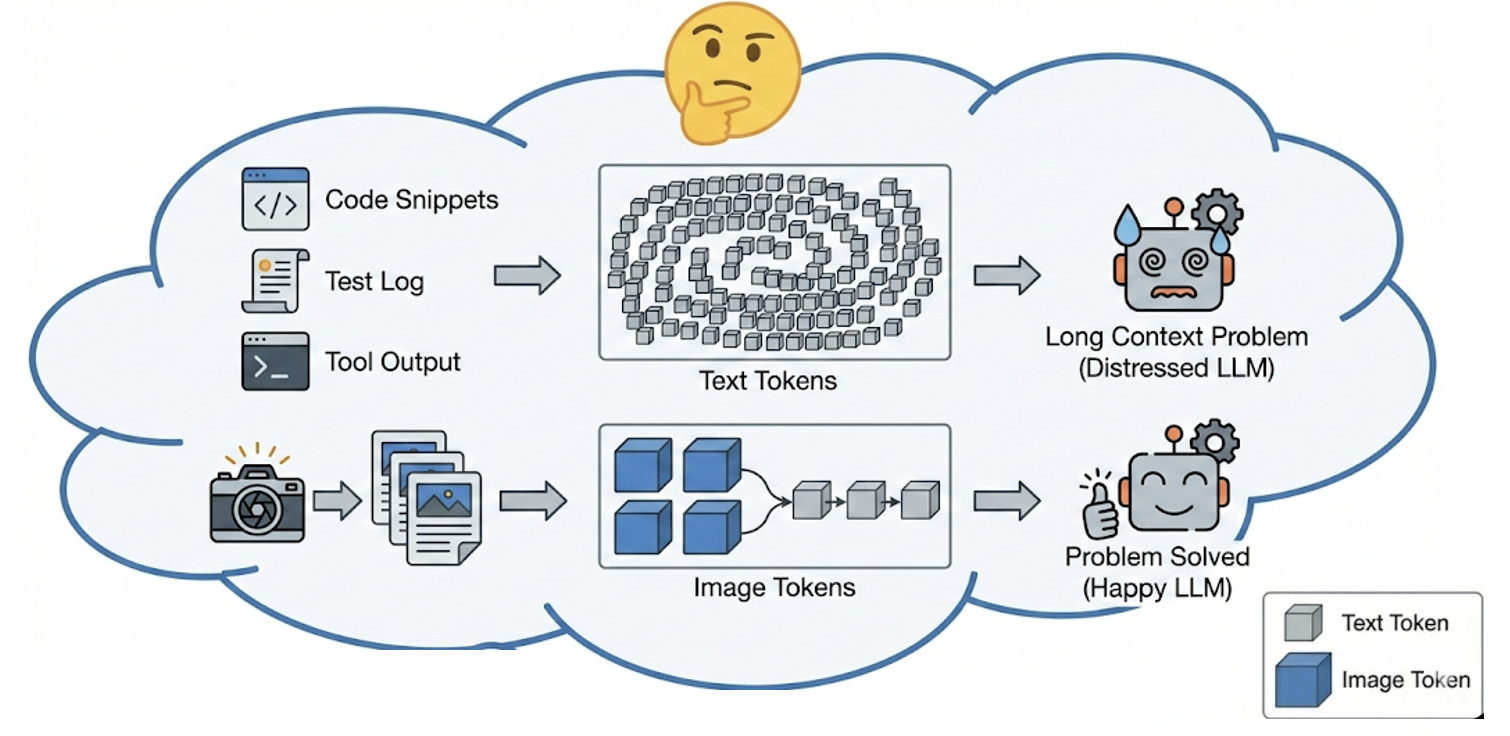
\includegraphics[width=\linewidth]{Sections/figures/overview.png}
  \caption{Overview of our main idea. Evaluating coding LLM on long context input: plain-text vs.\ ``OCR'' compression.}
  \vspace{-2em}
  \label{fig:overview}
\end{figure}


\para{Proposed Approach.}
As shown in Figure~\ref{fig:overview}, we evaluate optical compression as a drop-in replacement for text-based code context in an agentic coding pipeline. We build on mini-swe-agent \cite{yang2024sweagent} and implement an OpticalAgent that intercepts code-heavy tool outputs (identified by a simple heuristic) and renders them as monospace images before passing them to GPT-5-mini. The issue description and non-code outputs (error messages, directory listings, short search results) remain as text. This observation-level design ensures that the bulk of code the model reads, namely file contents accessed via file-reading commands, is presented as images.

\para{Experiments.}
We conducted a two-phase evaluation. First, a \emph{readability pilot study} swept rendering parameters (font sizes 8--20pt, page widths 100--140 characters) across six diverse Python code samples, establishing that GPT-5-mini achieves $\le$1.5\% character error rate and 100\% identifier recall at 12pt/120-character width. Second, we ran the full agentic pipeline on a 100-instance stratified subset of SWE-bench Verified, comparing the text baseline against the optical condition. We measured resolve rate, token usage, dollar cost, wall clock time, and behavioral differences.

\para{Results.}
We draw two main conclusions. First, \textbf{optical code input without any post-training is fully viable}: the vision-capable model reads and reasons about code from images as accurately as from text, achieving identical resolve rates (51/100 for both conditions), with 41 instances resolved by both and 10 unique to each. Second, \textbf{image tokens are currently more expensive than text tokens}: the optical agent consumes 29\% more input tokens and costs 1.9$\times$ more per instance (\$0.06 vs.\ \$0.03). Realizing the cost-saving potential of optical compression will likely require post-training to reduce the number of vision tokens per image, as explored by concurrent work such as DeepSeek-OCR \cite{wei2025deepseekocr}.

\para{Contributions.}
The main contributions of this work are:
\begin{itemize}[leftmargin=*]
  \item A readability pilot study establishing that GPT-5-mini can reliably read Python source code from rendered images (CER $\le$1.5\%, 100\% identifier recall), with an analysis of error patterns including the model's tendency to semantically rewrite regex rather than transcribe it.
  \item A controlled evaluation demonstrating that optical code input is a viable drop-in replacement for text in an agentic coding pipeline, achieving equivalent resolve rates (51\% vs.\ 51\%) on SWE-bench Verified without any post-training.
  \item An analysis showing that while feasible, optical encoding is currently more expensive per instance, suggesting that post-training (e.g., learned visual encoders) is needed to make optical compression cost-competitive.
\end{itemize}

\section{Proposed Technique}

\subsection{Approach Overview}

\para{Input \& Output.}
We study a long-context coding task in an agentic setting: given (i)~a natural-language issue description and (ii)~access to a software repository at a fixed snapshot, the model interacts with a shell environment over multiple turns, reading files, running tests, and editing code, to produce a patch that resolves the described issue \cite{jimenez2023swebench}. We build on mini-swe-agent \cite{yang2024sweagent}, a minimal agentic framework where the agent repeatedly queries a language model, executes bash commands, and observes the output.

\para{Main Idea.}
Our core idea is to replace the \emph{text} representation of code with an \emph{image} representation wherever the agent encounters source code during its workflow. Concretely, when a tool command returns a code-heavy output (e.g., reading a file via a shell command), we render that output as a monospace document image (see Figure~\ref{fig:rendering-example}) and present it to the vision-capable model as an image input instead of text. This lets us test whether a model can perform multi-step software engineering through the visual channel without any post-training or architectural change.

The key insight is that code reading happens predominantly during the agent loop, not in the initial problem description. Our analysis of agent traces shows that file-reading commands account for over 80\% of the code tokens the model processes, while code blocks in the issue description are a small fraction. Therefore, we apply optical encoding at the \emph{observation level}, intercepting tool outputs, rather than only at the input level.

\subsection{Approach Details}

\para{Observation-Level Optical Encoding.}
At each step of the agent loop, the model issues a bash command, the environment executes it, and the output is returned as a message. In the standard (text) setup, this output is a plain-text string. In our optical setup, we add an intermediate step: if the output is identified as code (see below), we render it as one or more images and present those images to the model in lieu of the text.

A technical constraint shapes the implementation: the OpenAI tool-call API requires tool-response messages to contain only text, not images. We work around this by (1)~replacing the code output in the tool message with a short placeholder (e.g., ``[Code output (243 lines) rendered as image in the next message]'') and (2)~injecting a follow-up user message containing the rendered images. The model thus sees the tool acknowledgment followed immediately by the visual code content.

\para{Code Detection Heuristic.}
Not all tool outputs should be rendered as images; directory listings, error messages, short grep results, and test outputs are better left as text. We apply a simple heuristic: an output is rendered as an image if and only if it satisfies both of the following conditions:
\begin{itemize}[leftmargin=*]
  \item \textbf{Length $>$ 2{,}000 characters}, ensuring that only substantial outputs are converted (short outputs gain little from compression).
  \item \textbf{Code ratio $>$ 20\%}, where ``code ratio'' is the fraction of lines whose stripped content starts with a Python keyword or indentation pattern (def, class, import, from, if, for, return, while, try, \#, or four-space indent).
\end{itemize}

Table~\ref{tab:code-detection-examples} illustrates the heuristic on representative tool outputs from our experiments. In practice, 25\% of all tool outputs are rendered as images (92 out of 366 across 20 pilot instances), and these account for the vast majority of code tokens the model processes.

\begin{table}[t]
\centering
\caption{Examples of the code detection heuristic. Outputs exceeding both thresholds (length $>$ 2{,}000 chars, code ratio $>$ 20\%) are rendered as images; others remain as text.}
\label{tab:code-detection-examples}
\small
\begin{tabular}{p{3.8cm}rrl}
\toprule
\textbf{Command} & \textbf{Chars} & \textbf{Code\%} & \textbf{Action} \\
\midrule
sed -n `1,240p' models.py & 7{,}859 & 31\% & Image \\
cat utils.py & 7{,}574 & 33\% & Image \\
python3 repro.py & 1{,}052 & 35\% & Text \\
grep -n ``def prepare'' & 87 & 0\% & Text \\
ls -la & 1{,}030 & 0\% & Text \\
git diff file.py & 1{,}268 & 6\% & Text \\
\bottomrule
\end{tabular}
\end{table}

\para{Rendering Pipeline.}
Each code output that passes the heuristic is rendered into one or more PNG images using the Python Pillow library. The rendering specification was determined through a systematic pilot study (Section~\ref{sec:rendering-config}): 12pt DejaVu Sans Mono, 120-character page width, 80 lines per image, black text on white background, no syntax highlighting. Files exceeding 80 lines are split across multiple images, each labeled with a header indicating the segment number.

% ------ Algorithm 1: Optical Encoding Pipeline ------
\begin{algorithm}[t]
\caption{Observation-Level Optical Encoding}\label{alg:optical}
\KwInput{Tool output text $t$, rendering parameters $\theta$}
\KwOutput{Message sequence $\mathcal{M}$ (tool message + optional image message)}
$r \leftarrow \mathrm{code\_ratio}(t)$\;
\uIf{$|t| > 2000$ \textbf{and} $r > 0.2$}{
  $n \leftarrow |\mathrm{lines}(t)|$\;
  $\mathit{chunks} \leftarrow \textsc{SplitByLines}(t,\; \theta.\mathit{max\_lines})$\;
  $\mathit{images} \leftarrow [\textsc{Render}(c, \theta) \text{ for } c \in \mathit{chunks}]$\;
  $m_{\mathrm{tool}} \leftarrow \text{``[Code output (}n\text{ lines) rendered as image]''}$\;
  $m_{\mathrm{img}} \leftarrow \textsc{UserMessage}(\mathit{images})$\;
  \Return{$(m_{\mathrm{tool}},\; m_{\mathrm{img}})$}
}{
  \Return{$(\textsc{ToolMessage}(t),)$} \tcp*{keep as text}
}
\end{algorithm}

Algorithm~\ref{alg:optical} summarizes the decision logic applied at each agent step. For outputs classified as code, the tool message contains a placeholder and a follow-up user message delivers the rendered images. For all other outputs, the original text is passed through unchanged.

\begin{figure}[t]
  \centering
  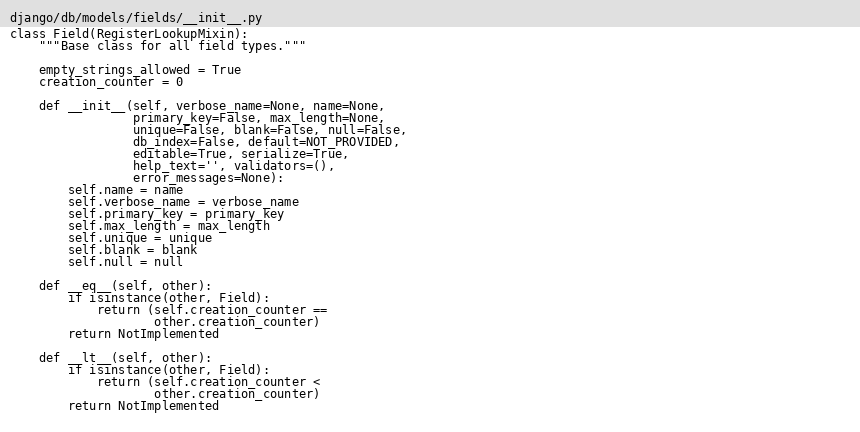
\includegraphics[width=\linewidth]{Sections/figures/rendering_example.png}
  \caption{Example of a rendered code image as seen by the model. The agent issued a file-read command; the output was detected as code (31\% code ratio, 7{,}859 characters) and rendered at 12pt/120-char width.}
  \label{fig:rendering-example}
\end{figure}

\para{Integration with mini-swe-agent.}
We implement the optical encoding as a subclass of the default agent (OpticalAgent) that overrides the action-execution method. The agent loop proceeds as follows: (1)~the model receives the conversation history and generates a bash command via tool call; (2)~the environment executes the command and returns the output; (3)~the OpticalAgent checks whether the output passes the code detection heuristic; (4a)~if yes, the output is rendered as images, the tool message is replaced with a placeholder, and a user message with the images is appended; (4b)~if no, the output is passed as text normally; (5)~the model sees the updated history and generates the next command. This cycle repeats until the model submits a patch or hits the step/cost limit.

This design requires no changes to the framework's core code, model interface, or environment layer. The same prompt template, decoding settings, and evaluation protocol are used for both conditions, ensuring that the input representation is the only experimental variable. The issue description (problem statement) is also preprocessed: markdown code blocks are rendered as images using the same pipeline.

\section{Experimental Evaluation}

We aim to answer the following research questions:
\begin{itemize}[leftmargin=*]
  \item \textbf{RQ1 (Fidelity).} How accurately can GPT-5-mini read Python source code from rendered images, and which code features are most error-prone?
  \item \textbf{RQ2 (Effectiveness).} Does providing code context as images affect patch success on SWE-bench Verified compared to plain-text context?
  \item \textbf{RQ3 (Efficiency).} How does optical encoding affect token usage, dollar cost, and wall clock time?
\end{itemize}

\subsection{Evaluation Setting}

\para{Benchmark and task.}
We evaluate on a 100-instance stratified subset of SWE-bench Verified \cite{openai2024swebenchverified}, drawn from all 12 repositories in the dataset using proportional allocation (see Appendix for the full instance list). Each instance provides a repository snapshot and a GitHub issue description; the agent must produce a patch that fixes the issue \cite{jimenez2023swebench}.

\para{Test-based evaluation.}
We apply each generated patch and run the benchmark's containerized test suite, following the official SWE-bench protocol: FAIL\_TO\_PASS tests must pass, and PASS\_TO\_PASS tests must remain passing \cite{jimenez2023swebench}.

\para{Model and agent.}
We use GPT-5-mini as the backbone model within the mini-swe-agent framework. The agent has a 50-step limit and a \$3 cost limit per instance. All other settings (prompt template, tool interface, environment) are identical across conditions.

\para{Conditions.}
We compare two conditions:
\begin{itemize}[leftmargin=*]
  \item \textbf{Text.} Standard setup where all tool outputs are returned as plain text.
  \item \textbf{Optical.} Code-heavy tool outputs (length $>$ 2{,}000 characters and code ratio $>$ 20\%) are rendered as monospace images and presented via a follow-up user message; all other outputs remain as text. Issue-description code blocks are also rendered as images.
\end{itemize}

\para{Prompt alignment.}\label{sec:prompt-alignment}
In an initial 20-instance pilot, we observed that image inputs caused GPT-5-mini to alter its workflow behavior: the model ran git commit before generating the patch in 85--90\% of optical runs versus only 10\% of text runs, causing git diff to return empty output. Table~\ref{tab:prompt-alignment} shows this effect and its resolution.

\begin{table}[t]
\centering
\caption{Prompt alignment pilot (20 instances). Adding an explicit ``do not commit'' instruction eliminates the behavioral divergence.}
\label{tab:prompt-alignment}
\small
\begin{tabular}{llccc}
\toprule
\textbf{Condition} & \textbf{Prompt} & \textbf{Git commit} & \textbf{Empty patch} & \textbf{Avg steps} \\
\midrule
Text          & before fix & 2/20 (10\%)  & 1/20 (5\%)  & 23.4 \\
Optical       & before fix & 17/20 (85\%) & 4/20 (20\%) & 20.1 \\
\midrule
Optical       & after fix  & 0/20 (0\%)   & 1/20 (5\%)  & 17.9 \\
\bottomrule
\end{tabular}
\end{table}

After adding the instruction ``Do NOT run git add or git commit; your changes must remain as uncommitted modifications,'' the commit behavior dropped to 0\% and the empty-patch rate matched the text baseline. All main experiments use the fixed prompt. This finding is noteworthy in its own right: multimodal inputs can alter model behavior in ways entirely unrelated to the content, a confound that must be controlled in any fair comparison. Apart from this directive and one additional system instruction for the optical condition (``Some code content may be provided as images''), both conditions use identical prompts.

\para{Metrics.}
For each instance $\times$ condition, we record: resolve status (pass/fail), total input and output tokens (summed across all agent steps), dollar cost, wall clock time (from first to last model query timestamp), number of agent steps, and, for the optical condition, the number of images rendered and the fraction of tool outputs rendered as images.

\para{Readability confirmation.}
The pilot study in Section~\ref{sec:rendering-config} establishes that GPT-5-mini can reliably read Python code from our rendered images: CER $\le$1.5\% on standard code, 100\% identifier recall, and 100\% indentation accuracy at the selected configuration (12pt, 120-character width). This confirms that downstream performance differences, if any, are not attributable to the model's inability to parse the images.


% ===================================================================
\subsection{Image Readability Pilot (RQ1)}\label{sec:rendering-config}
% ===================================================================

Before the main experiment, we conducted a pilot study to determine image rendering parameters that give the best fidelity-to-cost tradeoff. The question is: \emph{at what font size, page width, and image height can GPT-5-mini accurately read Python code from images?}

\para{Motivation.}
If the model cannot reliably recover code from images, any downstream performance difference would be uninterpretable, as we would not know whether failures stem from optical compression itself or from poor rendering choices. This section establishes a lower bound on image readability before proceeding to the main evaluation.

\para{Test samples.}
We analyzed the SWE-bench Verified dataset to understand code length distributions: the median patch is 22 lines and the 90th percentile is 77 lines. Guided by this, we selected six Python source code samples (46--155 lines) covering import-heavy modules, nested control flow with exception handling, and regex/special-character-heavy code.

\para{Metrics.}
For each rendering configuration, we prompted GPT-5-mini to transcribe the rendered image and compared the transcription against the ground truth using: character error rate (CER), identifier recall (fraction of Python names recovered), and indentation accuracy (fraction of matching lines with correct leading whitespace).

\para{Round 1: Font size sweep.}
We tested seven font sizes (8--20pt) at a fixed 100-character page width. Table~\ref{tab:fontsize-sweep} shows the results.

\begin{table}[t]
\centering
\caption{Font size sweep (page width = 100 chars, 80 lines/image). CER and token cost as a function of font size.}
\label{tab:fontsize-sweep}
\small
\begin{tabular}{lcccc}
\toprule
\textbf{Font} & \textbf{Avg CER} & \textbf{Id Recall} & \textbf{Indent Acc} & \textbf{Avg Tokens} \\
\midrule
f8   & 0.084 & 0.97 & 0.60 &  538 \\
f10  & 0.046 & 0.99 & 0.83 &  700 \\
\textbf{f12}  & \textbf{0.023} & \textbf{0.99} & \textbf{0.99} & \textbf{1{,}038} \\
f14  & 0.019 & 0.99 & 0.82 & 1{,}338 \\
f16  & 0.030 & 0.99 & 0.69 & 1{,}853 \\
f18  & 0.018 & 1.00 & 0.83 & 2{,}161 \\
f20  & 0.027 & 0.99 & 0.82 & 2{,}349 \\
\bottomrule
\end{tabular}
\end{table}

CER drops sharply from f8 (8.4\%) to f12 (2.3\%), indicating a threshold below which the vision encoder cannot resolve monospace characters. Above f14, CER does not consistently improve, while tokens scale linearly. Identifier recall remains $\ge$0.97 at all sizes. We selected \textbf{12pt}: CER within 0.4 percentage points of the best (18pt), at 52\% fewer tokens.

\para{Round 2: Page width and image height.}
Error analysis revealed that the dominant error at f12/w100 was \emph{line truncation}: lines exceeding 100 characters wrapped in the image, and the model reproduced the break. We tested wider pages (120, 140 chars) and taller images (120 lines). Table~\ref{tab:pagewidth} shows the results.

\begin{table}[t]
\centering
\caption{Effect of page width and image height on fidelity (at 12pt and 14pt).}
\label{tab:pagewidth}
\small
\begin{tabular}{lcccc}
\toprule
\textbf{Setting} & \textbf{CER} & \textbf{Indent} & \textbf{Id Recall} & \textbf{Tokens} \\
\midrule
f12, w100        & 0.023 & 0.99 & 0.99 & 1{,}038 \\
\textbf{f12, w120} & \textbf{0.023} & \textbf{1.00} & \textbf{1.00} & \textbf{1{,}160} \\
f14, w120        & 0.018 & 0.83 & 1.00 & 1{,}524 \\
f14, w140        & 0.015 & 0.83 & 1.00 & 1{,}762 \\
\midrule
f12, l120        & 0.025 & 0.83 & 0.99 & 1{,}009 \\
f14, l120        & 0.021 & 0.74 & 0.99 & 1{,}306 \\
\bottomrule
\end{tabular}
\end{table}

Widening to 120 characters eliminated truncation for $>$97\% of SWE-bench code lines and pushed indentation accuracy to 1.00 at f12. Further widening to 140 chars yielded marginal improvement at 52\% higher cost. Increasing image height from 80 to 120 lines \emph{worsened} quality: indentation accuracy dropped from 0.99 to 0.83, consistent with a ``lost at the bottom'' effect where the vision encoder loses fidelity in tall images.

\para{Error patterns.}
Two residual error modes persist at the selected configuration (f12, w120, 80 lines/image).

\emph{Regex rewriting.} The model does not transcribe complex regex patterns character-by-character; instead, it parses the pattern semantically and regenerates what it considers an equivalent expression. Table~\ref{tab:regex-rewrite} shows three examples from our test suite. In each case, the transcribed regex captures the same language class as the original but uses different grouping or quantifier syntax. This behavior inflates CER on regex-heavy code ($\sim$9\% vs.\ $\sim$1\% on standard code) but does not necessarily indicate a failure of understanding, as the model demonstrably comprehends the pattern's intent.

\begin{table}[t]
\centering
\caption{Regex rewriting: the model generates semantically similar but syntactically different expressions. Differences are underlined.}
\label{tab:regex-rewrite}
\small
\begin{tabular}{p{3.6cm}p{3.6cm}}
\toprule
\textbf{Ground truth} & \textbf{Transcription} \\
\midrule
\texttt{@(\textbackslash w+\ul{(?:\textbackslash.\textbackslash w+)*(?:\textbackslash([{\^{}})\linebreak]*\textbackslash))?})\textbackslash s*\$} &
\texttt{@(\textbackslash w+\ul{(\textbackslash.\textbackslash w+)*)\textbackslash s*(\textbackslash([{\^{}})\linebreak]*\textbackslash))?}\textbackslash s*\$} \\
\midrule
\texttt{{\^{}}(?:from\textbackslash s+\ul{([\textbackslash w.]+)}\textbackslash s+)?\linebreak import\textbackslash s+\ul{(.+)}\$} &
\texttt{{\^{}}\textbackslash s*(?:from\textbackslash s+\ul{[\textbackslash w\textbackslash.]+}\textbackslash s+)?\linebreak import\textbackslash s+\ul{[\textbackslash w\textbackslash*,\textbackslash s]+}} \\
\bottomrule
\end{tabular}
\end{table}

\emph{Header injection.} When content spans multiple images, the model occasionally inserts the header from the next image into the transcription output. This is a predictable, strippable artifact.

Table~\ref{tab:per-sample} shows per-sample CER at the final configuration.

\begin{table}[t]
\centering
\caption{Per-sample CER at f12/w120. Identifier recall is 1.00 for all samples.}
\label{tab:per-sample}
\small
\begin{tabular}{llcc}
\toprule
\textbf{Sample} & \textbf{Feature} & \textbf{Lines} & \textbf{CER} \\
\midrule
dense\_imports      & imports, dataclass    & 46  & 0.1\% \\
agent\_short        & class, type hints     & 50  & 1.5\% \\
special\_chars      & regex, escapes        & 58  & 9.4\% \\
complex\_logic      & nested logic, f-str   & 96  & 1.1\% \\
agent\_medium       & class, URLs           & 100 & 1.0\% \\
agent\_full         & full module           & 155 & 0.9\% \\
\bottomrule
\end{tabular}
\end{table}

\para{Selected configuration.}
We fix \textbf{12pt font, 120-character page width, 80 lines per image} for all subsequent experiments. This achieves CER $\le$1.5\% (excluding the regex outlier) with perfect indentation accuracy and identifier recall, at 1{,}160 tokens per sample.


% ===================================================================
\subsection{Main Results (RQ2, RQ3)}\label{sec:eval-results}
% ===================================================================

Table~\ref{tab:main-results} presents the main results on 100 SWE-bench Verified instances.

\begin{table}[t]
\centering
\caption{Main results: Text vs.\ Optical on 100 SWE-bench Verified instances.}
\label{tab:main-results}
\small
\begin{tabular}{lcc}
\toprule
\textbf{Metric} & \textbf{Text} & \textbf{Optical} \\
\midrule
Instances resolved       & 51/100 (51\%) & 51/100 (51\%) \\
Patches with content     & 96/100        & 98/100 \\
Limits exceeded          & 0             & 2 \\
\midrule
Avg input tokens         & 292{,}060     & 376{,}722 \\
Avg output tokens        & 5{,}143       & 5{,}596 \\
Avg images per instance  & n/a           & 14.5 \\
Avg agent steps          & 21.3          & 19.8 \\
Avg cost per instance    & \$0.03        & \$0.06 \\
Total cost (100 inst.)   & \$3.25        & \$6.25 \\
Avg wall clock (s)       & 120.8         & 165.0 \\
\bottomrule
\end{tabular}
\end{table}


\para{RQ2: Effectiveness.}
Both conditions resolve exactly 51 of 100 instances, yielding identical 51\% resolve rates. However, the resolved sets are not identical. Table~\ref{tab:overlap} breaks down the overlap.

\begin{table}[t]
\centering
\caption{Overlap analysis: instance-level agreement between Text and Optical.}
\label{tab:overlap}
\small
\begin{tabular}{lc}
\toprule
\textbf{Category} & \textbf{Count} \\
\midrule
Both resolved (agree)        & 41 \\
Neither resolved (agree)     & 39 \\
Text only (Text $>$ Optical) & 10 \\
Optical only (Optical $>$ Text) & 10 \\
\midrule
Total agreement              & 80/100 (80\%) \\
\bottomrule
\end{tabular}
\end{table}

The two conditions agree on 80\% of instances, with 10 instances uniquely solved by each. This symmetric disagreement pattern suggests that optical encoding does not systematically help or hurt: the model is equally capable of reasoning from either modality, but introduces different variance in each.

\para{Disagreement analysis.}
We examined the 20 disagreement instances for systematic patterns. The optical-only set is dominated by Django instances (7/10), compared to only 3/10 in the text-only set. The text-only set includes more instances from repositories with complex mathematical notation (Sympy: 3/10, xarray: 3/10). One hypothesis is that Django's highly standardized code style (consistent indentation, naming conventions, docstring patterns) is particularly well-suited to visual parsing, while mathematical/scientific code with dense symbolic expressions may lose precision in image rendering. However, the small sample size (10 per group) limits the statistical power of this comparison.

We also note that GPT-5-mini does not support temperature=0, so all outputs involve sampling noise. Some of the 20 disagreement instances may simply reflect run-to-run variance rather than genuine modality effects. Disentangling these factors would require multiple runs per instance per condition, which we leave to future work.

\para{RQ3: Efficiency.}
The optical condition is more expensive on every efficiency metric. Input tokens increase by 29\% (376K vs.\ 292K) because image tokens are less dense than text tokens: the same 240 lines of code that occupy $\sim$2{,}000 text tokens require $\sim$3{,}500 image tokens. Dollar cost nearly doubles (\$0.06 vs.\ \$0.03), reflecting both the higher token count and the typically higher per-token price of image inputs. Wall clock time increases by 37\% (165s vs.\ 121s), attributable to image rendering overhead and larger payloads.

However, the optical agent takes \emph{fewer} steps on average (19.8 vs.\ 21.3). One possible explanation is that code images provide a more visually salient overview of file structure, allowing the model to locate relevant sections faster. We note that this step reduction is not large enough to offset the per-step token increase.

These results highlight an important distinction: optical encoding is \emph{feasible} (equivalent task performance) but not yet \emph{cheaper}. The cost overhead stems from the current vision tokenization scheme, where image tokens are less dense than text tokens. Realizing actual cost savings would require post-training to compress vision token counts; for example, DeepSeek-OCR \cite{wei2025deepseekocr} achieves 10$\times$ compression ratios with a trained encoder, which could potentially make optical encoding cost-competitive or even cheaper than text.

\para{Code detection in the main experiment.}
In the optical condition, 25\% of tool outputs are classified as code and rendered as images (92/366 in the 20-instance pilot). On the full 100-instance run, the optical agent rendered an average of 14.5 images per instance. The code detection heuristic (length $>$ 2{,}000 chars and code ratio $>$ 20\%) produces very few false positives: only 3 out of 92 rendered outputs in the pilot were from non-standard commands (Python script executions whose output happened to contain code-like patterns), and all three were arguably appropriate to render.

The pilot study (Section~\ref{sec:rendering-config}) established that CER on standard Python code is $\le$1.5\% with 100\% identifier recall. The main experiment confirms that this fidelity level is sufficient: the 51\% resolve rate matches the text baseline, indicating that any character-level errors introduced by optical encoding do not materially affect the model's ability to understand code and generate correct patches.


\para{Case studies.}
We examine three instances to illustrate the qualitative differences between conditions.

\emph{Optical succeeds, text fails (django-13401):} The issue concerns Django's Field class ordering behavior. Both agents read the same source file, but followed different strategies. The optical agent (14 steps) performed targeted searches for equality and comparison methods and ran verification tests before submitting, producing a correct patch. The text agent (11 steps) applied a patch more quickly but skipped edge-case verification, resulting in a patch that failed the test suite. This suggests that the visual layout may have helped the optical agent perceive the method structure more holistically, leading to more thorough verification.

\emph{Text succeeds, optical fails (django-11532):} The issue involves a change in Django's database backend. The text agent (12 steps) identified and fixed the issue correctly. The optical agent (16 steps) read the same code and produced a patch of similar length, but the fix was subtly incorrect, as the generated patch did not fully address the test requirements. This illustrates that while optical encoding preserves code readability, the model's reasoning from visual input can occasionally diverge, leading to different (and sometimes wrong) solution paths.

\emph{Both succeed, different paths (astropy-14995):} Both agents resolved this Astropy issue, but the optical agent did so in 13 steps compared to the text agent's 21 steps, a 38\% reduction. Inspecting the trajectories, the text agent explored several unrelated files before locating the correct one, while the optical agent navigated more directly. The optical agent processed 7 code images (versus raw text), yet arrived at the correct fix faster. This case illustrates the ``fewer steps'' trend observed in the aggregate data (19.8 vs.\ 21.3 average steps) and suggests that the spatial layout of code images may sometimes aid navigation efficiency, even though the overall token cost is higher.

\section{Related Work}

\para{Long-context handling for coding LLMs.}
Repository-level coding benchmarks such as SWE-bench cast software engineering as generating a patch for a real GitHub issue given a full codebase snapshot and an execution-based test oracle \cite{jimenez2023swebench,openai2024swebenchverified}. Agentic systems typically mitigate the resulting long-context burden through three complementary strategies. First, \emph{retrieval}: systems such as SWE-agent \cite{yang2024sweagent}, Agentless \cite{xia2024agentless}, and AutoCodeRover \cite{zhang2024autocoderover} search for relevant files, functions, or code snippets and present only these to the model, avoiding the need to pass the entire repository as context. Second, \emph{pruning and selection}: agents discard low-utility lines, constrain editable regions, or truncate long tool outputs to fit within context budgets \cite{yao2022react,schick2023toolformer}. Third, \emph{summarization and compression}: methods like LLMLingua replace long observations with model-generated summaries or compressed prompts to reduce token counts \cite{jiang2023llmlingua}. Retrieval-augmented generation is also a standard paradigm for selecting supporting context under a budget \cite{lewis2020rag,karpukhin2020dpr,robertson2009bm25}, and in code-centric settings, repository-level retrieval and representation learning are commonly used to identify relevant files or snippets \cite{zhang2023repocoder,feng2020codebert,guo2020graphcodebert,guo2022unixcoder}. Orthogonally, recent work on extending context windows through positional encoding modifications (e.g., RoPE scaling \cite{su2024rope}) and efficient attention mechanisms \cite{dao2022flashattention} has pushed context limits to 128K+ tokens, but these approaches do not reduce the per-token cost of processing long inputs. Our work explores a different axis: changing the \emph{modality} of long code context from text to images.

\para{Optical compression via image encoding.}
A separate line of work explores representing long textual contexts through the visual channel: text is rendered into a 2D layout and consumed as an image so that a vision-capable model can decode or reason over it with a smaller (or differently priced) input representation \cite{openai2023gpt4v_systemcard,shi2023gpt4v_ocr,kim2021donut,lee2022pix2struct}. DeepSeek-OCR explicitly frames this as \emph{contexts optical compression}, training a specialized encoder to keep the number of vision tokens manageable under high-resolution inputs while retaining decodability \cite{wei2025deepseekocr}. AgentOCR applies optical representations to compress agent interaction histories, showing that rendering prior tool outputs as images can reduce context length without significantly degrading task performance \cite{feng2026agentocr}. In the document understanding domain, models such as Nougat \cite{blecher2023nougat} and Pix2Struct \cite{lee2022pix2struct} are trained end-to-end to parse rendered document images, achieving strong results on scientific papers and web pages. Importantly, most reported gains in this space rely on specialized training or tailored visual encoders, leaving open how much benefit can be obtained \emph{without} post-training when applying optical encoding to code-centric artifacts \cite{wei2025deepseekocr,feng2026agentocr}.

\para{Vision-capable LLMs for code tasks.}
Vision-language models such as GPT-4V \cite{openai2023gpt4v_systemcard} and its successors have demonstrated the ability to read and reason about code from screenshots, UI mockups, and handwritten notes. Several studies have benchmarked these models on code-from-image tasks: for example, generating code from UI screenshots \cite{si2024design2code} or understanding code structure from rendered images \cite{shi2023gpt4v_ocr}. However, these evaluations typically focus on the model's vision capability as a \emph{standalone skill}---asking the model to read and reproduce code from an image in a single turn. Our work differs in that we use vision as an \emph{input channel within a multi-step agentic workflow}: the model must not only read code from images but also reason about it, plan edits, and generate patches over many turns of interaction. This places different demands on the vision encoder, requiring sustained fidelity across dozens of images per episode rather than one-shot transcription accuracy.

\para{Agentic coding and observation formatting.}
The design of the agent-computer interface (ACI) has been shown to significantly affect agentic coding performance. SWE-agent \cite{yang2024sweagent} introduced the concept of ACI design, demonstrating that the format in which tool outputs are presented to the model---including truncation, line numbering, and context windowing---can substantially change resolve rates. The ReAct framework \cite{yao2022react} established the interleaved reasoning-and-acting paradigm that most coding agents follow, while Reflexion \cite{shinn2023reflexion} showed that feeding back execution observations in structured formats improves self-correction. Our work contributes to this line by demonstrating that the \emph{modality} of observation formatting (text vs.\ image) is another axis of ACI design, and that changing this modality can alter model behavior in unexpected ways (Section~\ref{sec:prompt-alignment}), even when the underlying information content is preserved.

\para{Multimodal inputs and model behavior.}
An emerging body of work studies how the presence of multimodal inputs affects LLM behavior beyond the content of those inputs. Studies have shown that including images in prompts can alter the model's tone, verbosity, and instruction-following behavior, even when the images are irrelevant to the task \cite{gong2023figstep}. Our finding that image inputs cause GPT-5-mini to systematically change its git workflow (committing before diffing, Section~\ref{sec:prompt-alignment}) is consistent with this phenomenon: the presence of visual content appears to shift the model's behavioral distribution in ways that are independent of the image content itself. This suggests that multimodal agentic systems require careful prompt alignment to control for modality-induced behavioral confounds, a consideration that has received limited attention in the agentic coding literature.

\para{How our study differs.}
Rather than proposing a new trained compressor, we provide a controlled evaluation of optical encoding as a \emph{pure input representation change} for agentic coding. We test a fixed vision-capable model (GPT-5-mini) on SWE-bench Verified and compare text against optical input at the observation level, where the agent reads code through tool outputs. Unlike DeepSeek-OCR \cite{wei2025deepseekocr} and AgentOCR \cite{feng2026agentocr}, we require no post-training; unlike document understanding models \cite{blecher2023nougat,lee2022pix2struct}, we evaluate on a downstream software engineering task rather than transcription accuracy alone. Our study is, to our knowledge, the first to evaluate optical compression for code in an agentic software engineering setting with a full execution-based evaluation.

\begin{table}[t]
\centering
\caption{Comparison with related approaches.}
\label{tab:related-work}
\small
\begin{tabular}{p{2.0cm}cccc}
\toprule
& \textbf{Post-train} & \textbf{Code} & \textbf{Agentic} & \textbf{Zero-shot} \\
\midrule
LLMLingua \cite{jiang2023llmlingua}       & No  & No  & No  & Yes \\
DeepSeek-OCR \cite{wei2025deepseekocr}    & Yes & No  & No  & No  \\
AgentOCR \cite{feng2026agentocr}          & Yes & No  & Yes & No  \\
Nougat \cite{blecher2023nougat}           & Yes & No  & No  & No  \\
Agentless \cite{xia2024agentless}         & No  & Yes & No  & Yes \\
\textbf{Ours}                             & No  & Yes & Yes & Yes \\
\bottomrule
\end{tabular}
\end{table}

\section{Threats to Validity}

\para{Internal validity.}
Our code detection heuristic (code ratio $>$ 20\%, length $>$ 2{,}000 characters) is a simple rule that may produce false positives (rendering non-code outputs as images) or false negatives (missing code outputs). In our 20-instance pilot, only 3 of 92 rendered outputs were borderline cases (Python script outputs), and manual inspection confirmed they contained code-like content. A more sophisticated classifier could improve precision, but would introduce its own complexity and potential confounds.

The image rendering pipeline introduces design choices---font size, page width, line wrapping---that were fixed via the pilot study. A different specification might yield different results. We mitigate this by selecting parameters that achieve near-perfect fidelity ($\le$1.5\% CER, 100\% identifier recall) and documenting the selection process transparently.

GPT-5-mini does not support \texttt{temperature=0}, so all outputs involve sampling noise. The 10/10 symmetric disagreement between conditions may partly reflect this randomness rather than genuine modality differences. Multiple runs per instance would be needed to disentangle these effects.

\para{External validity.}
We evaluate a single model (GPT-5-mini) on a single benchmark (100-instance subset of SWE-bench Verified). Our findings may not generalize to other vision-capable LLMs with different vision encoders or to other coding tasks beyond patch generation. SWE-bench Verified is predominantly Python; optical encoding may behave differently for other languages with different visual density or indentation conventions.

\para{Construct validity.}
The SWE-bench pass rate is binary: a patch either passes all required tests or fails. This does not capture partial correctness or near-miss patches. Our cost comparison depends on current OpenAI API pricing, which may change. The code detection heuristic's thresholds (2{,}000 chars, 20\% code ratio) were chosen empirically and not optimized; different thresholds could shift the balance of what gets rendered.

\section{Conclusion}

We evaluated optical compression---rendering source code as monospace images---as a drop-in replacement for text-based code input in an agentic software engineering pipeline. On a 100-instance subset of SWE-bench Verified using GPT-5-mini, the optical condition matched the text baseline exactly (51\% resolve rate each), with 80\% instance-level agreement and a symmetric 10/10 split of unique successes.

We draw two main conclusions. First, \textbf{optical code input without post-training is fully viable}: GPT-5-mini's vision encoder can read and reason about Python source code from rendered images with the same effectiveness as from text. Our readability pilot confirms this at the character level ($\le$1.5\% CER, 100\% identifier recall), and the main experiment confirms it at the task level (identical resolve rates). This result is encouraging for the broader vision of optical compression: the fundamental capability is already present in current vision-capable models.

Second, \textbf{image tokens are currently more expensive than text tokens}, so optical encoding does not yet deliver cost savings. The optical agent consumed 29\% more input tokens and cost 1.9$\times$ more per instance (\$0.06 vs.\ \$0.03). This overhead arises because current vision tokenizers produce more tokens per unit of information than text tokenizers. Bridging this gap will likely require post-training to compress vision token counts---concurrent work such as DeepSeek-OCR \cite{wei2025deepseekocr} achieves 10$\times$ compression ratios with a trained encoder, which could make optical encoding not only feasible but cost-competitive.

\para{Contributions.}
\begin{itemize}[leftmargin=*]
  \item A readability pilot study establishing GPT-5-mini's code-reading fidelity from images, including the discovery that the model semantically rewrites regex patterns rather than transcribing them.
  \item A controlled comparison demonstrating that optical code input achieves equivalent resolve rates to text in an agentic setting without any post-training, establishing feasibility.
  \item An analysis showing that while feasible, optical encoding is currently more expensive, motivating future work on trained visual encoders to achieve cost-competitive optical compression.
\end{itemize}

\para{Future work.}
The most impactful next step is to combine our zero-shot optical encoding with a trained visual encoder (e.g., DeepSeek-OCR \cite{wei2025deepseekocr} or AgentOCR \cite{feng2026agentocr}) that reduces vision token counts, potentially achieving both the feasibility demonstrated here and actual cost savings. Other directions include: evaluating on additional models (Gemini, Claude) to test generalizability; hybrid approaches that render only long outputs as images while keeping short outputs as text; multiple runs per instance to disentangle modality effects from sampling noise; and extending to other languages and task types (code completion, test generation).


\balance
\bibliographystyle{ACM-Reference-Format}
\bibliography{reference}

\appendix
\section{Transcription Prompt}
The following prompt was used in the image readability pilot (Section~\ref{sec:rendering-config}) to evaluate GPT-5-mini's code-reading fidelity:

\begin{quote}
\small\texttt{Transcribe the exact text content shown in this image. Preserve all whitespace, indentation, symbols, and formatting exactly as shown. Do not add any explanation or commentary --- output ONLY the transcribed text.}
\end{quote}

\section{Instance Selection}
The 100-instance subset was constructed from SWE-bench Verified using proportional stratified sampling across all 12 repositories (seed=42). Table~\ref{tab:repo-dist} shows the allocation. The full list of instance IDs and the selection script (\texttt{scripts/build\_subset\_100.py}) are available in the artifact repository.

\begin{table}[h]
\centering
\caption{Repository distribution of the 100-instance subset.}
\label{tab:repo-dist}
\small
\begin{tabular}{lr|lr}
\toprule
\textbf{Repository} & \textbf{N} & \textbf{Repository} & \textbf{N} \\
\midrule
django       & 44 & pydata/xarray   & 4 \\
sympy        & 15 & pytest-dev      & 4 \\
sphinx-doc   &  9 & psf/requests    & 2 \\
matplotlib   &  7 & pylint-dev      & 2 \\
scikit-learn &  6 & mwaskom/seaborn & 1 \\
astropy      &  5 & pallets/flask   & 1 \\
\bottomrule
\end{tabular}
\end{table}


\end{document}
